\documentclass{beamer}
\mode<presentation>{\usetheme{Madrid}}

\usepackage[T1]{fontenc}
\usepackage[utf8]{inputenc}
\usepackage{hyperref}
\usepackage{multicol}
\usepackage{animate}%per gif

\definecolor{mygreen}{RGB}{54, 219, 95}

\setbeamertemplate{caption}[numbered]%per numerare immagini
\hypersetup{
    %colorlinks=true,
    linkcolor=black,
    filecolor=magenta,      
    urlcolor=blue,
}

\title{GOOGLE RESEARCHES}
\subtitle{An awesome \LaTeX presentation}
\date{UpdateUpgrade: STB1019}
\author{Stefano Prandini, 13/03/2018}

\begin{document}

\AtBeginSection[]%stampa table of contents ogni sezione
{
\begin{frame}<beamer>
\frametitle{What Now?}
%\footnotesize
\begin{multicols}{2}
  \tableofcontents[currentsection]
\end{multicols}
\end{frame}
}
\AtBeginSubsection[]%stampa table of contents ogni sottoSezione
{
\begin{frame}<beamer>
\frametitle{What Now?}
%\footnotesize
\begin{multicols}{2}
\tableofcontents[currentsection, currentsubsection]
\end{multicols}
\end{frame}
}

\begin{frame}
\titlepage%genera il titolo
\end{frame}

\begin{frame}{Chi siamo}
\begin{figure}[h!]
\begin{center}

\includegraphics[width=\linewidth]{immagini/stb-unibs.png}
\end{center}
\end{figure}
\end{frame}

\begin{frame}{Chi sono}
\begin{center}
Androidified \textbf{Stefano Prandini\\}
\animategraphics[loop,controls,width=0.5\linewidth]{20}{immagini/stefanogif/stefano-}{0}{50}%gif, si vede solo con adobe
\end{center}
\end{frame}

\begin{frame}{Google Search}
\begin{figure}[h!]
\begin{center}

\includegraphics[width=\linewidth]{immagini/motore-di-ricerca-google.jpg}
\end{center}
\end{figure}
\end{frame}

\begin{frame}{TABLE OF CONTENTS}%indice iniziale
%\footnotesize
\begin{multicols}{2}
\tableofcontents
\end{multicols}
\end{frame}


\section{PREFAZIONE}
\begin{frame}{PREFAZIONE}
\begin{figure}[h!]
\begin{center}

\includegraphics[width=0.4\linewidth]{immagini/ricerca-felicit.jpg}
\caption{Gli uomini si dividono in due categorie: quelli che cercano il senso della vita senza trovarlo e quelli che l'hanno trovato senza cercarlo [cit. Emil Cioran]}
\end{center}
\end{figure}
\end{frame}

\subsection{What?}
\begin{frame}{What?}
\footnotesize
\begin{itemize}
\item Questo incontro è finalizzato al fornirvi metodologie di ricerca online più efficaci del semplice "scrivere una parola/frase su Google", in modo che i risultati ottenuti possano essere più veloci e soddisfacenti.\\ 
\item L'importanza di questo incontro risiede più nel concetto (effettuare ricerche dettagliate) che nel contenuto (come farlo): \\
I contenuti avreste infatti potuto trovarli tramite ricerche su internet.
\end{itemize}
%\begin{multicols}{2}
\begin{figure}[h!]
\begin{center}

\includegraphics[width=80pt]{immagini/uroboros.jpg}
\begin{center}\caption {Cercare su internet come cercare su internet inizia a diventare in qualche modo ricorsivo, \textit{quindi ecco questa presentazione.}}\end{center}
\end{center}
\end{figure}
%\end{multicols}
\end{frame}

\subsection{Why?}
\begin{frame}{Why?}
\newtheorem{thm}{\begin{center}Easy Theorem\end{center}}
\begin{thm}<1->
Spesso molte domande ("tecniche") che vengono poste potrebbero essere rimpiazzate da una sana ricerca mirata su internet, facendo risparmiare tempo a tutti.
\end{thm}
\end{frame}


\section{GET STARTED}
\begin{frame}{GET STARTED}
\begin{block}{\begin{center}Definizione\end{center}}
\begin{center}"Google è un ragazzotto di 20 anni"\end{center}
\end{block}
\begin{block}{\begin{center}All'anagrafe\end{center}}
\begin{center}Google Search, 15/09/1997, Stanford.\\ Partorito da Larry Page e Sergey Brin.\end{center}
\end{block}
\begin{figure}[h!]
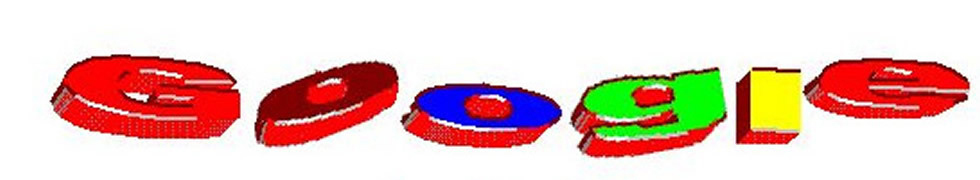
\includegraphics[width=0.8\linewidth]{immagini/google11.jpg}
\caption{Primo, abominevole, logo di google. 1997-1998}
\end{figure}
\end{frame}
\begin{frame}{GET STARTED}
\begin{block}{\begin{center}Fun Fact\end{center}}
Larry e Sergey volevano chiamare il loro motore di ricerca "Googol", ispirandosi al numero chiamato \textit{googol}\footnote{Termine coniato da Edward Kasner nel 1938, nel suo libro Matematica e immaginazione: "numero intero esprimibile con 1 seguito da cento zeri"}, pensando fosse il termine perfetto per rappresentare l'immensa quantità di informazioni disponibili sul Web: al momento della registrazione del dominio si accorsero di non sapere come fosse scritto, finendo per scrivere "Google"\footnote{Fonte: "The Google Story" di David A. Vise}.\\
\end{block}
\end{frame}
\begin{frame}{GET STARTED}
\begin{center}
\begin{figure}[h!]

\includegraphics[width=\linewidth]{immagini/Googol.png}
\caption{Un \textit{Googol}, a.k.a. 10 000 000 000 000 000 000 000 000 000 000 000 000 000 000 000 000 000 000 000 000 000 000 000 000 000 000 000 000 000 000 000 000 000 $= 10^{100}$. }
\end{figure}
\end{center}
\end{frame}


\section{MATEMATICA DI GOOGLE}
\begin{frame}{MATEMATICA DI GOOGLE}
\textbf{Come il motore di ricerca considera il web:} Il Web viene pensato come un enorme grafo, ossia una sorta di ragnatela i cui fili sono i collegamenti (link) tra le pagine e i nodi tra i vari fili sono le pagine.\newline\newline
In particolare, dato un insieme di pagine Web $\{Pi\}_{i=1…n}$ si definiscono:
\begin{itemize}
\item la matrice di adiacenza $M_{adj} = (m_{adj})_{i,j}$:
\begin{equation*}
    (m_{adj})_{i,j} := 
    \begin{cases}
      1 & \text{se}\ \exists \text{ collegamento tra}\ P_i \text{ e } P_j \\
      0 & \text{otherwise}
    \end{cases}
  \end{equation*}
\item la matrice di transizione $M_{adj} = (m_{adj})_{i,j}$:
\begin{equation*}
    (m_{adj})_{i,j} := 
    \begin{cases}
      \frac{1}{|P_i|} & \text{se}\ \exists \text{ collegamento tra}\ P_i \text{ e } P_j \\
       0 & \text{otherwise}
    \end{cases}
  \end{equation*}
dove $|P_{i}|$ rappresenta il numero totale delle pagine a cui punta la pagina $P_{i}$.
\end{itemize}
\end{frame}
\begin{frame}
\begin{figure}[h!]

\includegraphics[width=0.9\linewidth]{immagini/nobodyCares.jpg}
\end{figure}
\end{frame}


\section{RICERCA AVANZATA}
\begin{frame}{RICERCA AVANZATA}
\begin{block}{\begin{center}What?\end{center}}
Restringi i risultati di ricerca per le ricerche complesse utilizzando la pagina Ricerca avanzata. Ad esempio, puoi trovare siti aggiornati nelle ultime 24 ore o immagini in bianco e nero.
\end{block}
\end{frame}

\subsection{Advanced Search}
\begin{frame}{Advanced Search}
\begin{center}Here: 
\footnotesize
\textcolor{blue}{\href{https://www.google.com/advanced_search}{https://www.google.com/advanced\_search}}
\begin{figure}[h!]
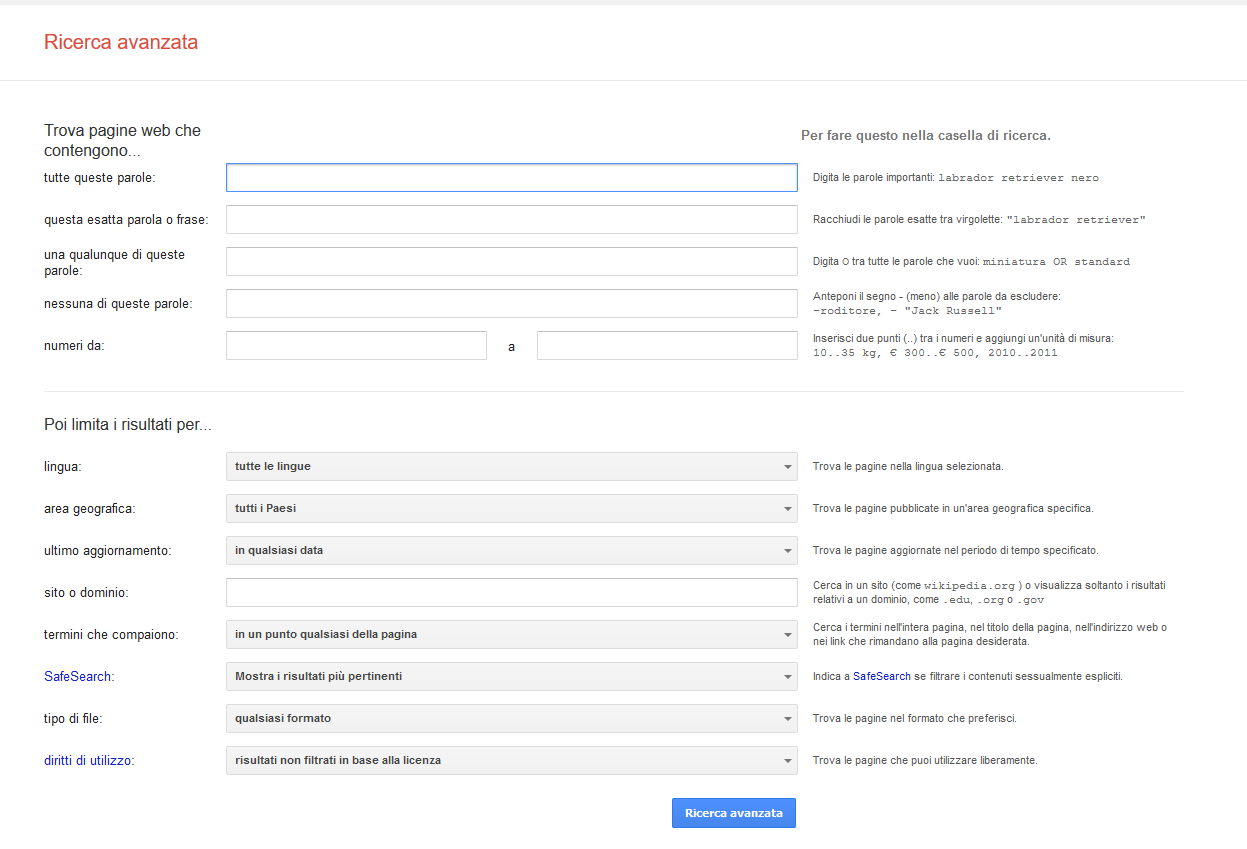
\includegraphics[height=200pt]{immagini/advancedsearch.png}
\end{figure}
\end{center}
\end{frame}
\begin{frame}{Advanced Search}
Filtri di ricerca avanzata che è possibile utilizzare:
\begin{itemize}
\item    Lingua
\item    Area geografica
\item    Ultimo aggiornamento (data)
\item    Sito o dominio
\item    Dove compaiono i termini di ricerca nella pagina
\item    SafeSearch
\item    Tipo di file (estensione)
\item    Diritti di utilizzo
\end{itemize}
\end{frame}

\begin{frame}{Advanced Search}
\begin{center}
\textit{Lingua, Area geografica, Ultimo aggiornamento, Sito o dominio, Tipo di file}: sappiamo tutti cosa sono
\end{center}
\begin{figure}[h!]

\includegraphics[width=0.7\linewidth]{immagini/hope.jpg}
\end{figure}
\end{frame}

\begin{frame}{Advanced Search}
\begin{block}{\begin{center}Campo "Dove compaiono i termini"\end{center}}
\begin{itemize}
\item \begin{center}Nel titolo della pagina\end{center}
\item \begin{center}Nel testo della pagina\end{center}
\item \begin{center}Nell'URL della pagina\end{center}
\item \begin{center}Nei link che rimandano alla pagina desiderata\end{center}
\end{itemize}
\end{block}
\end{frame}

\begin{frame}{Advanced Search}
\begin{block}{\begin{center}Campo "Safe search"\end{center}}
Google permette di filtrare i risultati di ricerca espliciti, ad esempio i contenuti pornografici, utilizzando l'impostazione SafeSearch.\\ SafeSearch non garantisce una precisione al 100\%, ma aiuta a evitare la visualizzazione di contenuti espliciti.
\end{block}
\begin{figure}[h!]

\includegraphics[width=0.33\linewidth]{immagini/18+.jpg}
\caption {(Utile in caso qualcuno di voi avesse figli di età [0-18[ anni)}
\end{figure}
\end{frame}
\begin{frame}{Advanced search}
\footnotesize
\begin{block}{\begin{center}Diritto di utilizzo\end{center}}
Non tutti i contenuti che si trovano su internet sono liberamente utilizzabili: questo campo nella ricerca avanzata consente di verificare se puoi utilizzare, condividere o modificare i \underline{contenuti trovati online}.\\ Essi possono essere:
\begin{itemize}
\item \textbf{Liberamente utilizzabili o condivisibili:} possono essere copiati o ridistribuiti, a condizione che non vengano modificati.
\item \textbf{Liberamente utilizzabili, condivisibili o modificabili:} possono essere copiati, modificati o ridistribuiti, secondo le modalità specificate nella licenza.
\item \textbf{A scopo commerciale:} possono essere utilizzati anche per scopi commerciali.
\end{itemize}
\end{block}
\end{frame}
\begin{frame}{Advanced Search}
Il diritto di utilizzo è da rispettare solo per un utilizzo dei contenuti che non rientri nel "Fair use": esso comprende scopi d'informazione, critica o insegnamento: in questi ambiti non è necessaria l'autorizzazione scritta da parte di chi detiene i diritti. \\
Il filtro va quindi utilizzato se l'utilizzo dei contenuti sarà per scopi professionali/commerciali.\\
\footnotesize 
\begin{block}{Un po' di legge:}
\begin{itemize}
\item Il \textit{Fair use} è una disposizione legislativa USA
\item Il governo italiano ha affermato che a seguito dell'entrata in vigore del decreto legislativo 9 aprile 2003, n. 68 («Attuazione della \textbf{direttiva 2001/29/CE»}), il testo dell'\textbf{articolo 70} della legge italiana sul diritto d'autore riprodurrebbe sostanzialmente il regime del fair use statunitense
\end{itemize}
\end{block}
\end{frame}

\subsection{Advanced Image Search}
\begin{frame}{Advanced Image Search}
\begin{center}Here: 
\footnotesize
\textcolor{blue}{\href{https://www.google.it/advanced_image_search}{https://www.google.com/advanced\_image\_search}}
\begin{figure}[h!]
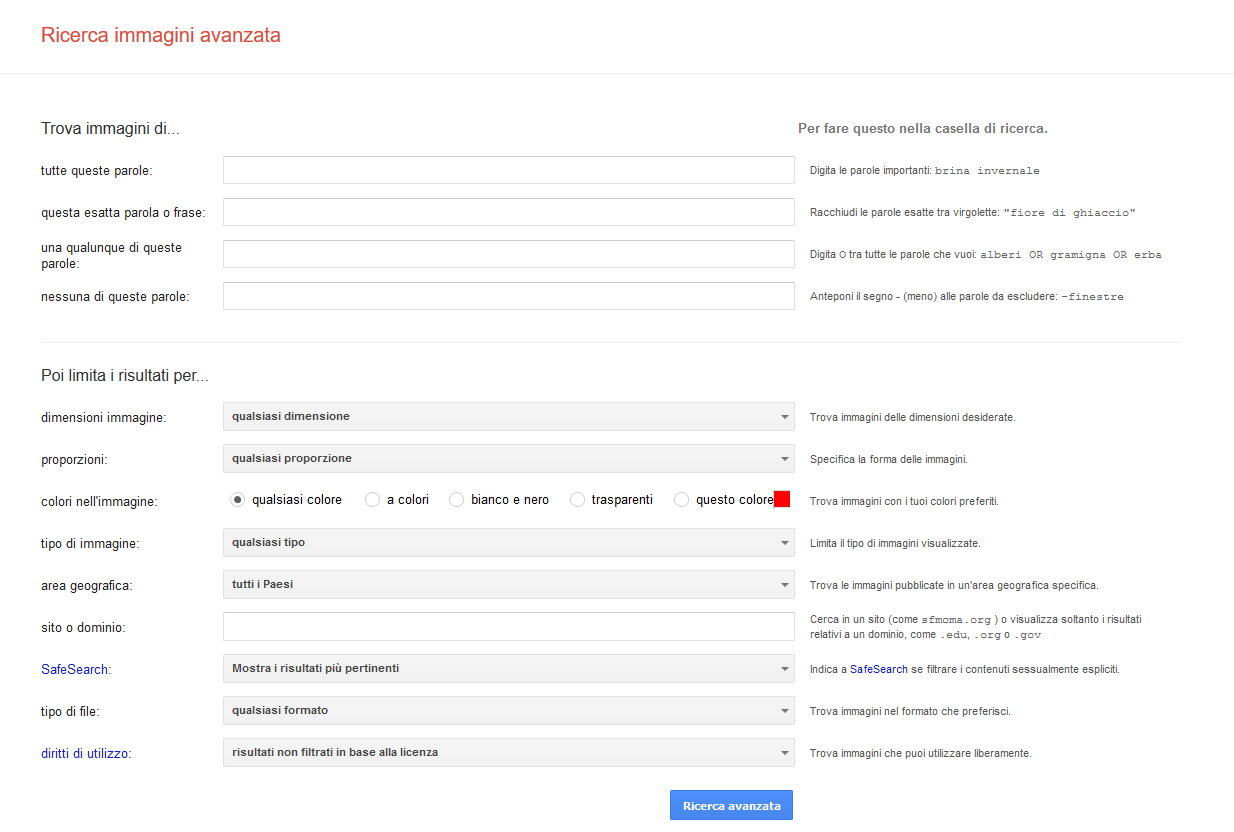
\includegraphics[height=200pt]{immagini/imageSearch.png}
\end{figure}
\end{center}
\end{frame}
\begin{frame}{Advanced Image Search}
Filtri di ricerca avanzata che è possibile utilizzare:
\begin{itemize}
\item    Dimensioni
\item    Proporzioni
\item    Colore
\item    Tipo
\item    Sito o dominio
\item    Tipo di file (estensione)
\item    SafeSearch
\item    Diritti di utilizzo
\end{itemize}
\end{frame}
\begin{frame}{Advanced Image Search}
\begin{block}{\begin{center}Campo "Tipo di immagine"\end{center}}
\begin{itemize}
\item Volti
\item Foto
\item Clip Art
\item Disegni
\item Animate
\end{itemize}
\end{block}
\end{frame}
\begin{frame}{Advanced Image Search}
\begin{figure}[h!]
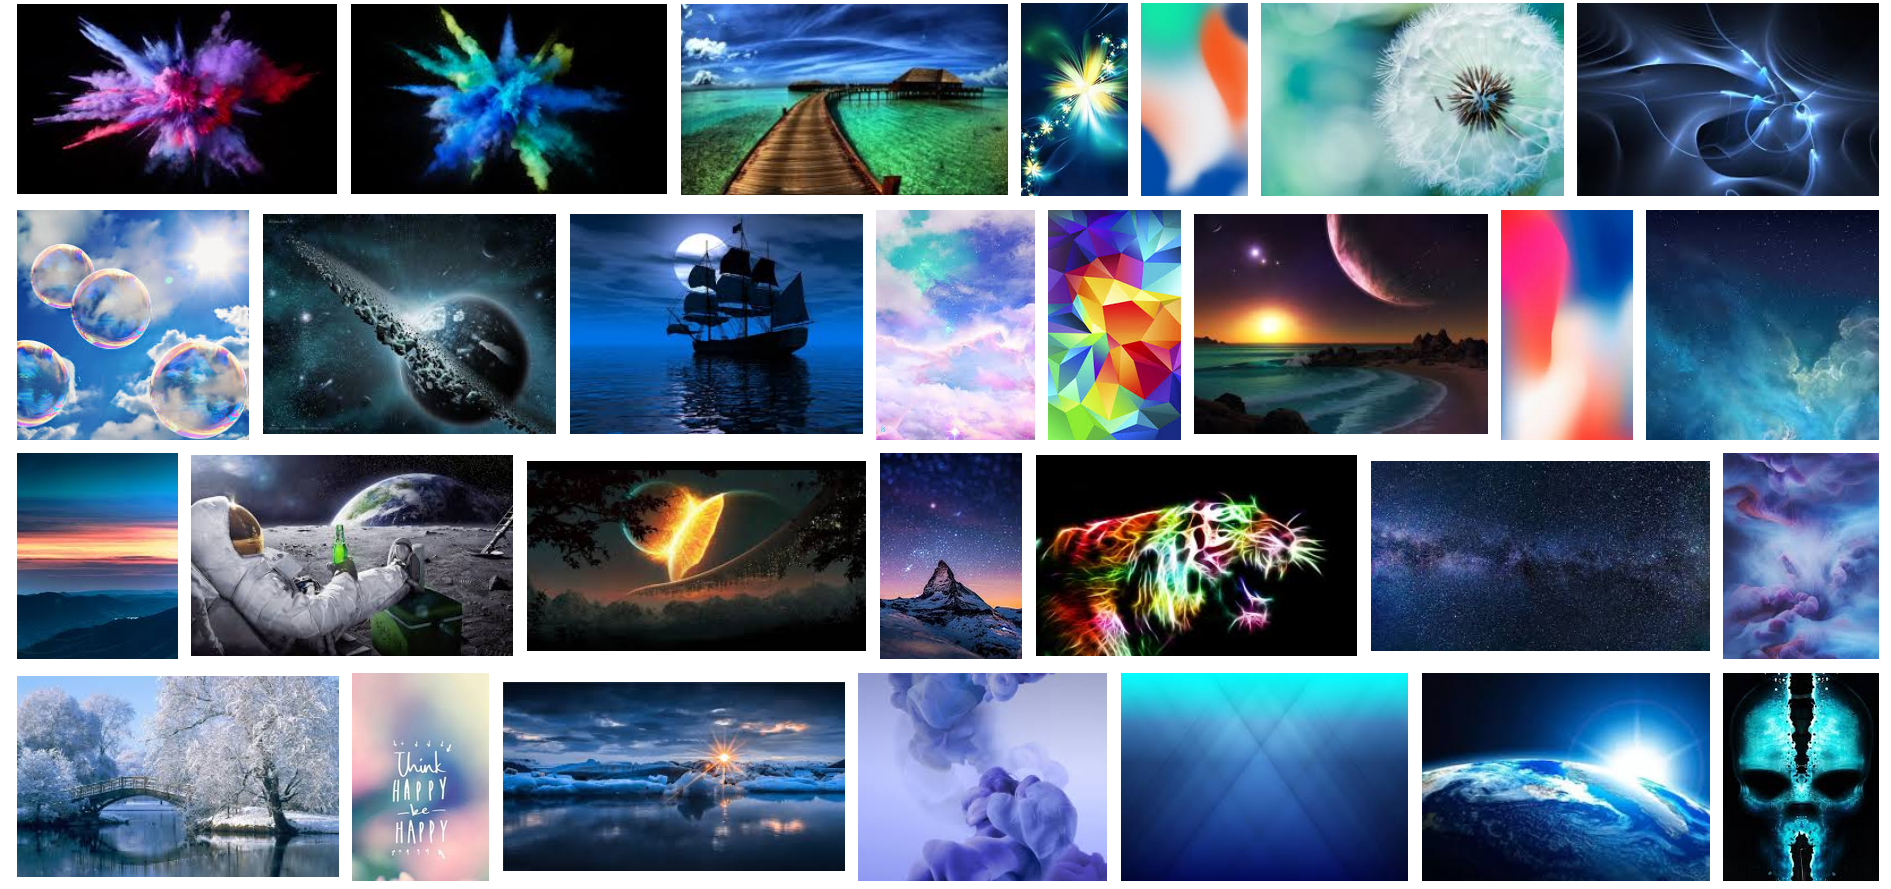
\includegraphics[width = \linewidth]{immagini/sfondi.png}
\caption {Ottimo per trovare immagini per articoli/relazioni/\textit{presentazioni bellissime come questa} (o sfondi)}
\end{figure}
\end{frame}

\section{COMANDI GOOGLE}
\begin{frame}{COMANDI GOOGLE}
Direttamente nella barra di ricerca, Google permette l'utilizzo dei cosiddetti "Comandi Google" (una serie di codici che permettono ricerche approfondite all'interno del motore di ricerca).
\newline\newline
Per esempio $"Define + termine"$ fornisce la definizione del termine cercato direttamente dal dizionario.
\end{frame}

\subsection{Cercare nelle parti di un sito}
\begin{frame}{Cercare nelle parti di un sito}
\footnotesize
\begin{itemize}
\item "\underline{Allintext}:parola1 parola2"\\fornisce la lista delle pagine indicizzate da Google che contengono delle determinate parole all'interno del \textbf{testo}.
\item "\underline{Allintitle}:parola1 parola2"\\fornisce la lista delle pagine indicizzate da Google che contengono delle determinate parole all'interno del \textbf{titolo}.
\item "\underline{Allinanchor}:parola1 parola2"\\fornisce la lista delle pagine indicizzate da Google che contengono delle determinate parole all'interno dell'\textbf{anchor}\footnote{il testo cliccabile di un link} dei link che la reindirizzano (es. "webmaster inanchor:giorgiotave" mostra le pagine linkate tramite l'anchor \textit{giorgiotave} e che contengono la key \textit{webmaster}).
\item "\underline{Allinurl}:parola1 parola2"\\fornisce la lista delle pagine indicizzate da Google che contengono delle determinate parole all'interno dell'\textbf{URL}.
\end{itemize}
(NOTA: è importante non inserire spazi tra le parole e i ":")
\end{frame}
\begin{frame}{Cercare nelle parti di un sito}
\begin{itemize}
\item I comandi preceduti da \textit{\underline{all}} cercano le parole che seguono il comando \textit{in qualsiasi ordine.}
\item Se si vuole cercare una frase precisa, essa va indicata tra apici (es. intext:"ricette di cucina").
\item Se si utilizzano i comandi senza \textit{\underline{all} (intext, intitle, inanchor, inurl)}, verrà cercato nel campo indicato solamente il termine che segue il comando, mentre gli altri verranno cercati in qualsiasi punto della pagina.
\end{itemize}
\end{frame}

\subsection{Escludere parole dalla ricerca}
\begin{frame}{Escludere parole dalla ricerca}
\begin{block}{\center{Operatore "-"}}
L'operatore "-" esclude i testi che contengono una certa parola chiave:\\ es. «inurl\footnote{visto prima}:ieeesb.unibs -"Stefano Prandini"» ricerca le pagine del nostro sito nelle quali non compare il mio nome (ma, per esempio, ci sono quelle che includono Stefano Poma\footnote{(se ci sei) ciao Stefano, bel nome}).
\end{block}
\end{frame}

\subsection{Cercare una corrispondenza esatta}
\begin{frame}{Cercare una corrispondenza esatta}
\begin{block}{\center{Operatore doppie virgolette}}
Se il testo è racchiuso fra doppie virgolette, Google ricerca le pagine Web che contengono esattamente la sequenza di caratteri digitata, senza altri spazi o caratteri intermedi.\\ es. «"student branch" "Stefano Prandini"» ricerca le pagine di tutti gli student branch (deve esserci la stringa esatta "Student branch") che contengono il mio nome (ma non quello di Stefano Poma\footnote{Non è sempre tutto rose e fiori}).
\end{block}
\end{frame}

\subsection{Usare caratteri/parole "jolly"}
\begin{frame}{Usare caratteri/parole "jolly"}
\begin{block}{\center{Operatore "*"}}
L'operatore jolly è il simbolo di asterisco.\\Es. «inurl:ieeesb.unibs "Stefano *"» restituisce le pagine del nostro dominio che contengono la parola Stefano seguita da un'altra qualsiasi (per esempio \textit{Stefano Prandini o Stefano Poma}).\\
Come \textit{carattere jolly} funziona solo se posto alla fine di una parola (caval* va bene, cava*lo no)
\end{block}
\end{frame}

\subsection{Altri comandi}
\begin{frame}{Altri comandi}
\begin{itemize}
\item \textbf{Combinare ricerche:}\\
Inserisci \underline{OR} tra ciascuna query di ricerca.\\ $\rightarrow$ Esempio: maratona OR gara.
\item \textbf{Cercare all'interno di siti specifici:}\\
Scrivi "\underline{site:}" davanti a un sito o un dominio.\\ $\rightarrow$ Esempio: "site:ieeesb.unibs.it", "site:.unibs.it" o "site:.gov".\\
(con "site:.unibs.it emanuele poggi" ho scoperto che il buon Poggi non ha passato l'appello V di Algebra nel 2016/2017, però ha passato Probabilità e statistica il 10/07/17)
\item \textbf{Cercare siti correlati:}\\
Scrivi "\underline{related:}" davanti a un indirizzo web che già conosci.\\ $\rightarrow$ Esempio: "related:unibs.it" reindirizza a unige.it, unimi.it, unipd.it,\ldots
\end{itemize}
\end{frame}

\subsection{Google Hacking}
\begin{frame}{Google Hacking}
\begin{block}{Non solo "pour parler"}
Molti di questi concetti non sono fini a loro stessi: chiunque può utilizzarli come meglio crede.  \\Un esempio? $\rightarrow$ \textit{Google Hacking}.
\end{block}
\medskip \textbf{Google Hacking} è una tecnica di "raccolta informazioni" che sfrutta gli strumenti che la ricerca avanzata di Google mette a disposizione: alcune query di ricerca possono essere utilizzate per identificare vulnerabilità di sicurezza nelle applicazioni Web, raccogliere informazioni su individui specifici (o casuali), rilevare messaggi di errore che rivelano informazioni sensibili, rilevare file contenenti credenziali e altri dati sensibili.
\end{frame}

\begin{frame}{Esempi: immagini/foto}
\begin{columns}
\begin{column}{0.5\textwidth}
\begin{itemize}
\item intitle:"index of"$^1$ photos
\item intitle:"index of" private
\item intitle:"index of" DCIM    
\end{itemize}   
\end{column}
\begin{column}{0.5\textwidth}
\begin{center}
\includegraphics[width=0.8\textwidth]{immagini/immagini.png}
\end{center}
\end{column}
\end{columns}
\medskip
\footnotesize
$^1$Restituisce un elenco di file archiviati su un server
\end{frame}

\begin{frame}{Esempi: mp3}
\begin{itemize}
\item \begin{center}intitle:"index of" mp3 metallica\end{center}
\end{itemize}
\begin{columns}
\begin{column}{0.5\textwidth}
\begin{center}
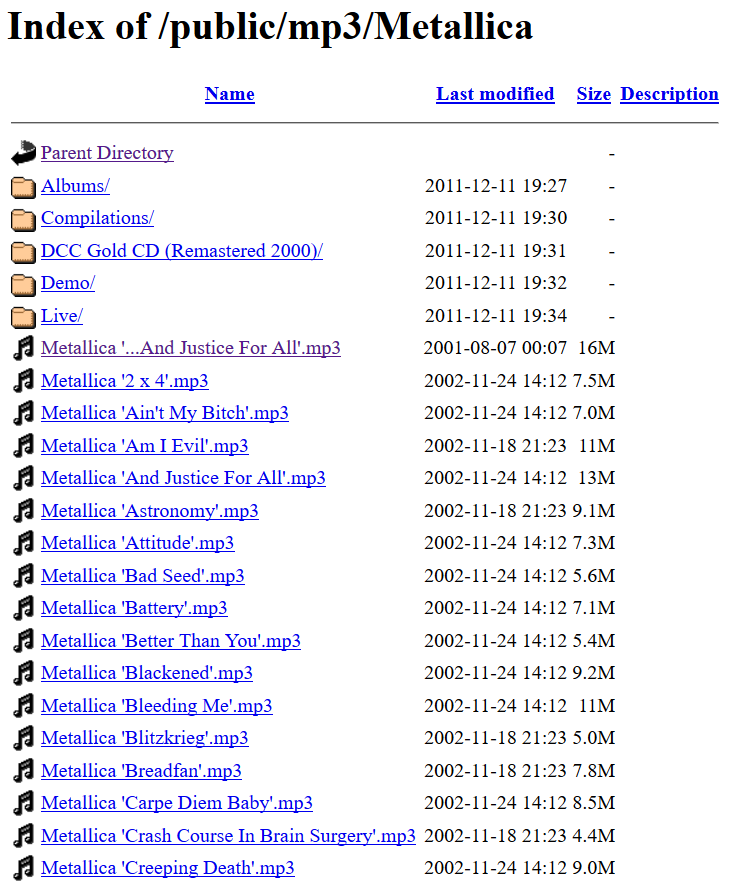
\includegraphics[width=\textwidth]{immagini/metallica.png}     
\end{center}
\end{column}
\begin{column}{0.5\textwidth}  
\begin{center}
     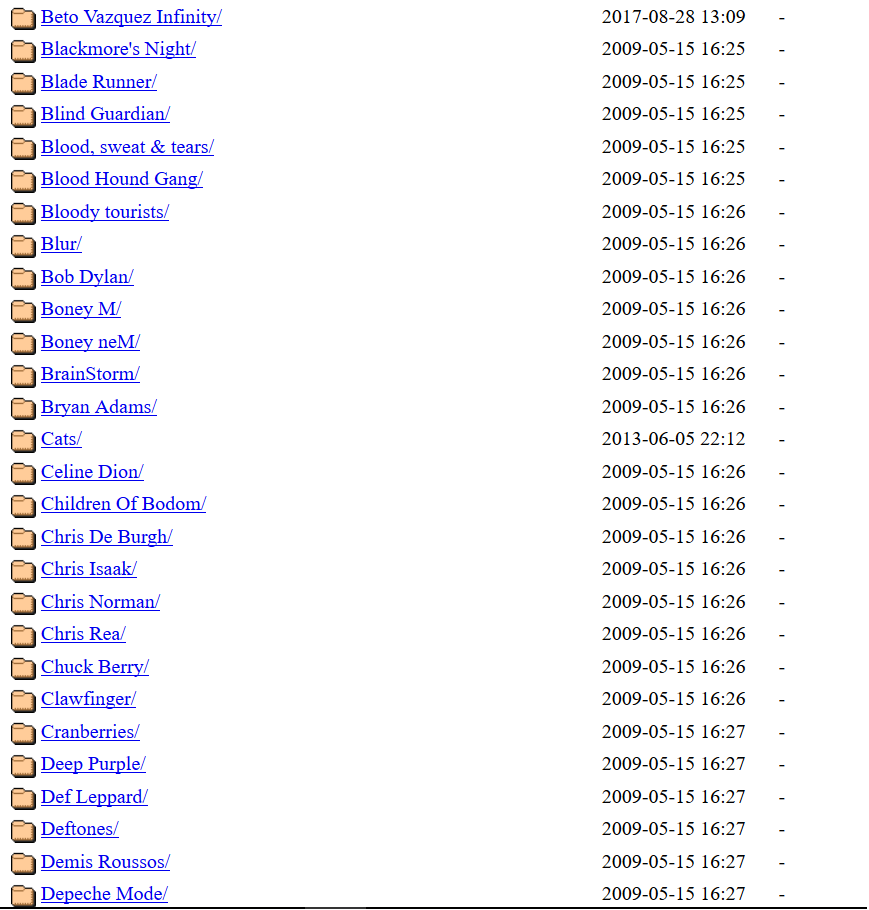
\includegraphics[width=0.9\textwidth]{immagini/list.png}
\end{center}
\end{column}
\end{columns}
\end{frame}

\begin{frame}{Esempi: webcam}
\begin{itemize}
\item \begin{center}intitle:"Live View / - AXIS"\end{center}
\item \begin{center}inurl:"viewerframe?mode=refresh"\end{center}
\item \begin{center}intitle:"Web Monitor" inurl:"simple.htm"\end{center}
\end{itemize}
\begin{figure}[h!]
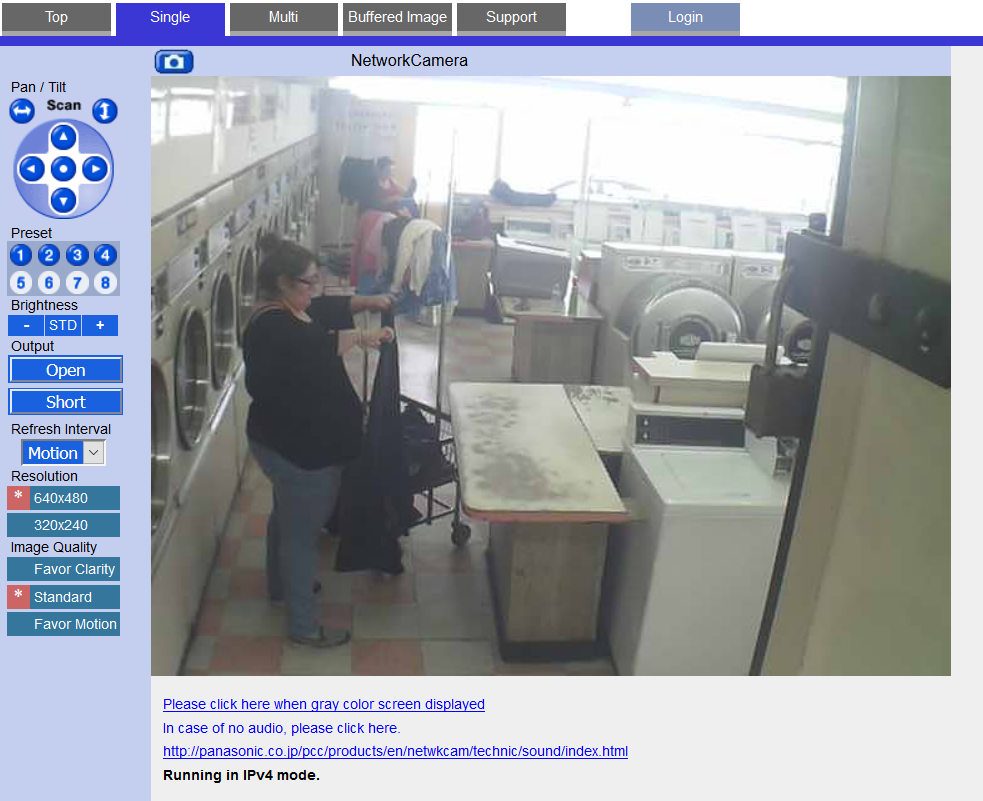
\includegraphics[width = 0.5\linewidth]{immagini/webcam.png}
\caption{interessantissima lavanderia in Vietnam}
\end{figure}
\end{frame}

\begin{frame}{Io Robot}
Dopo alcune ricerche "insolite" Google potrebbe chiedervi se siate umani
\begin{columns}
\begin{column}{0.6\linewidth}
\begin{figure}[h!]
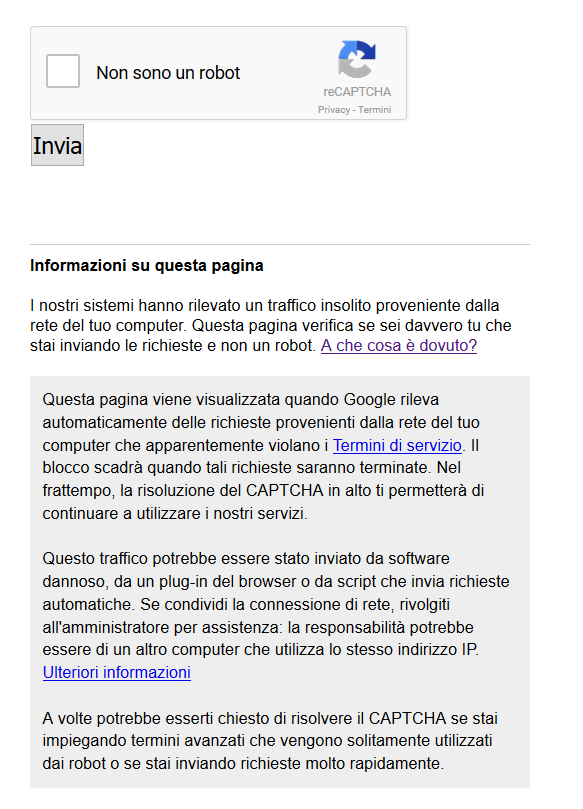
\includegraphics[height=0.7\textheight]{immagini/captcha.png}
\end{figure}
\end{column}
\begin{column}{0.3\linewidth}
\begin{figure}[h!]

\includegraphics[width=0.8\linewidth]{immagini/robot.jpg}
\end{figure}
\end{column}
\end{columns}
\end{frame}

\section{STRUMENTI GOOGLE}
\begin{frame}{STRUMENTI GOOGLE}
\begin{figure}[h!]

\includegraphics[height=0.6\textheight]{immagini/google-app.png}
\end{figure}
Vedremo ora gli \textbf{strumenti Google} fondamentali nella vita quotidiana e all'interno del Branch (che consentono di cooperare con maggiore facilità).
\end{frame}

\subsection{Google Scholar}
\begin{frame}{Google Scholar}
\begin{figure}[h!]

\includegraphics[width=0.5\linewidth]{immagini/scholar.png}
\end{figure}
\begin{block}{\center{Motto:}}
\begin{center}
\textit{"stand on the shoulders of giants"}\\
$[cit.\ Hegel\ [cit.\ Newton\ [cit.\ Giovanni\ di\ Salisbury]]]$\\
\end{center}
\center{(riferendosi alla possibilità di elevarsi nelle conoscenze e nelle competenze, aperta dalla migliore accessibilità della letteratura accademica)}
\end{block}
%Google ha introdotto l'I10-index per stimare l'affidabilità di un autore. (in aggiunta al già conosciuto H-index)
\end{frame}
\begin{frame}{Google Scholar}
\textit{Google Scholar} è un motore di ricerca (come Google Search) specializzato nell'individuazione di testi/articoli della \underline{"letteratura accademica"} (tesi di laurea, dottorato, libri, sommari, recensioni, rapporti tecnici di tutti i settori della ricerca scientifica, ...): se essi sono disponibili liberamente sul web verrano mostrati.\\
\medskip L'\textit{$\mathrm{I}$10-index}\footnote{indica il numero di pubblicazioni di un autore che hanno ricevuto almeno dieci citazioni} è stato introdotto da Google proprio all'interno di Scholar, aggiungendosi al già presente \textit{H-index}\footnote{uno scienziato ha un H-index di n se almeno n lavori tra quelli che ha pubblicato sono stati citati almeno n volte ciascuno (considera pubblicazioni e citazioni)}, per stimare l'affidabilità di un autore.
\end{frame}

\subsection{Google Trends}
\begin{frame}{Google Trends}
\begin{figure}[h!]

\includegraphics[width=0.5\linewidth]{immagini/trends.png}
\end{figure}
\medskip Strumento Google che permette di conoscere la \underline{frequenza di ricerca} sul web di una determinata parola o frase (specificando data e luogo), tramite un grafico che sintetizza l'andamento della sua popolarità.
\end{frame}
\begin{frame}{Google Trends}
\begin{figure}[h!]
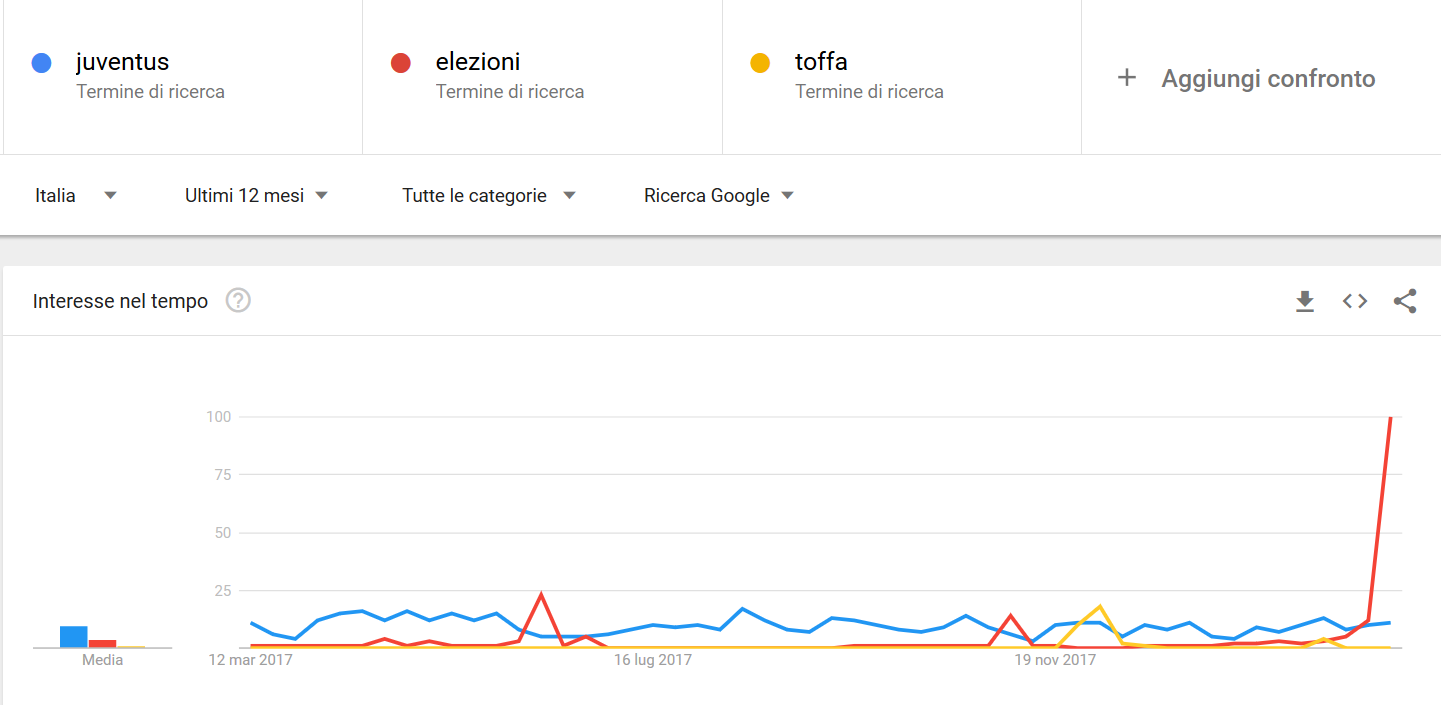
\includegraphics[width=0.85\linewidth]{immagini/trend.png}
\end{figure}
\footnotesize
\begin{columns}
\begin{column}{0.5\linewidth}
\begin{itemize}
\item 03/06/2017: finale Champions League "Juventus - Real Madrid"
\item 13/08/2017: finale Supercoppa Italiana "Juventus - Lazio"
\end{itemize}
\end{column}
\begin{column}{0.5\linewidth}
\begin{itemize}
\item 11/06/2017: elezioni amministrative
\item 05/11/2017: elezioni regionali Sicilia
\item 04/03/2018: elezioni politiche e regionali
\end{itemize}
\end{column}
\end{columns}
\end{frame}

\subsection{Google Calendar}
\begin{frame}{Google Calendar}
\begin{columns}
\begin{column}{0.5\linewidth}
\begin{figure}[h!]
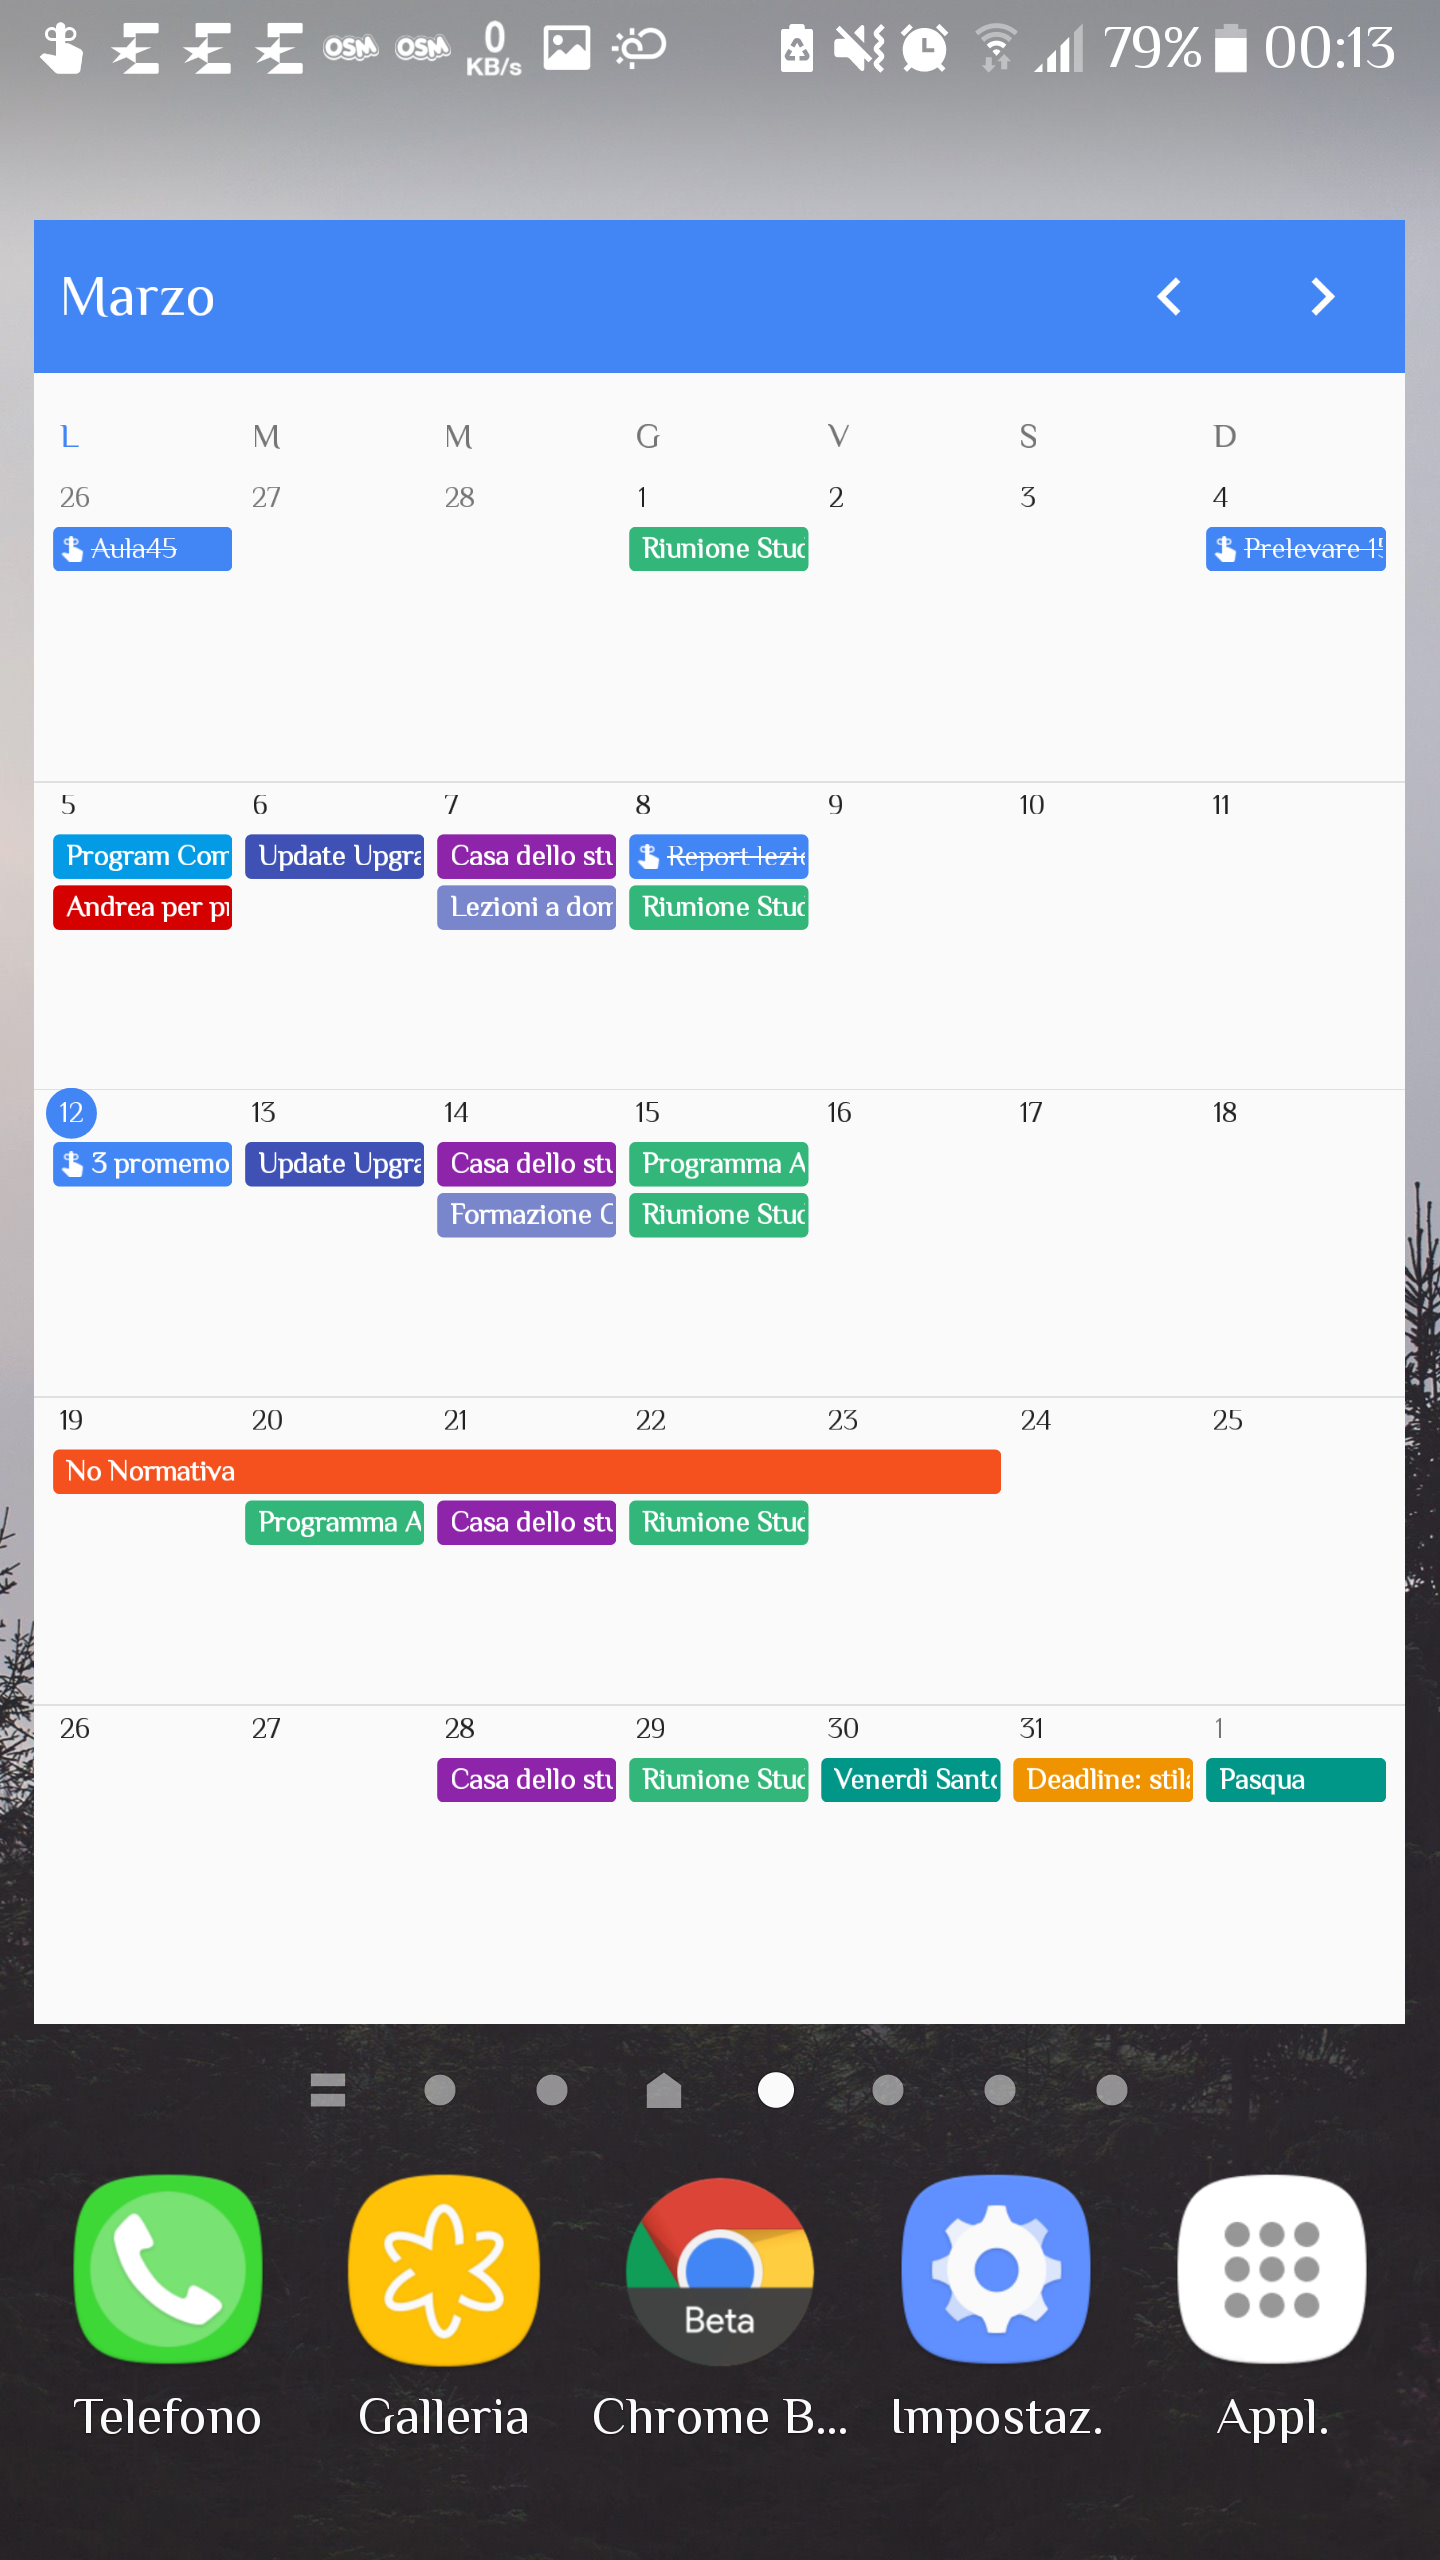
\includegraphics[height=0.8\textheight]{immagini/calendar.png}
\end{figure}
\end{column}
\begin{column}{0.5\linewidth}
\footnotesize
Il \textit{\underline{Google Calendar}} viene usato per segnare tutte le date degli incontri (o delle scadenze) che riguardano il Branch: esse vengono sempre comunicate anche tramite email, ma averle sott'occhio\footnote{per gli utenti Android $\rightarrow$ widget} (anche belle colorate) è sempre utile. Inoltre dovrebbe arrivare anche una notifica il giorno prima dell' "evento".\\Questa applicazione \underline{non} deve dunque mancare sui vostri smartphone: il suo utilizzo è semplice e può aiutarvi anche nei vostri impegni personali.
\end{column}
\end{columns}
\end{frame}

\subsection{Google Keep}
\begin{frame}{Google Keep}
\begin{columns}
\begin{column}{0.5\linewidth}
\begin{figure}[h!]
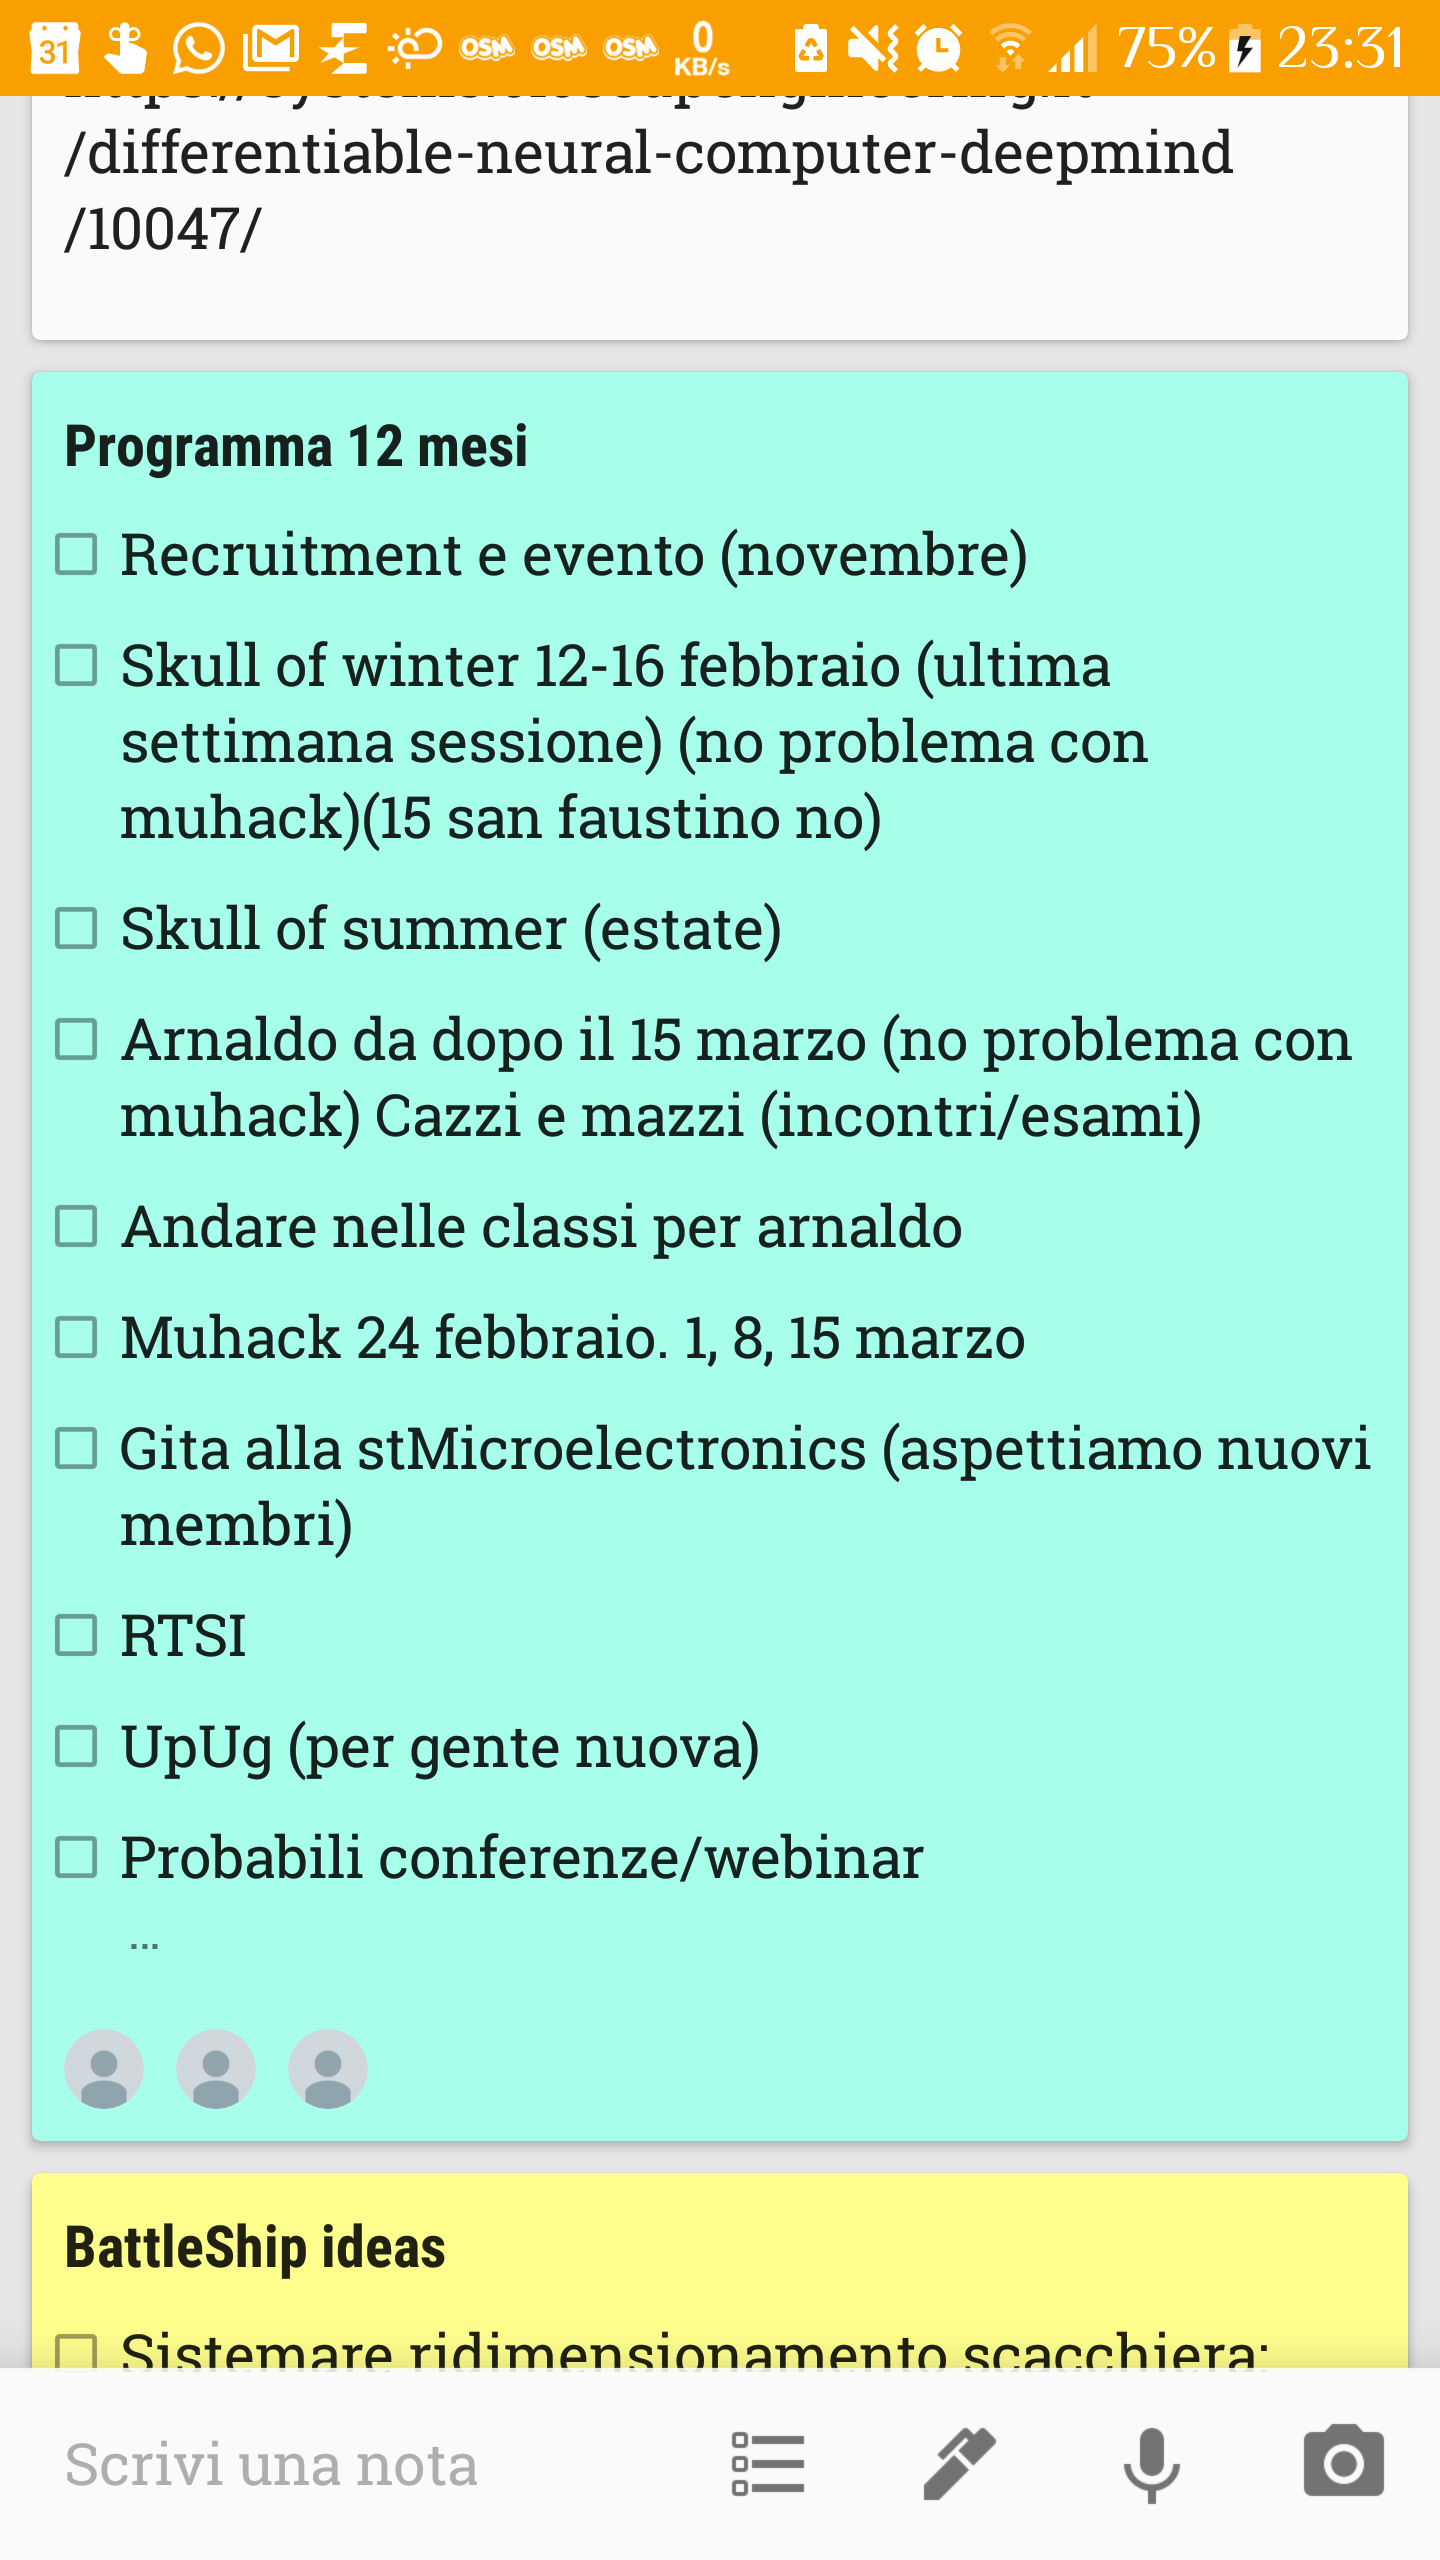
\includegraphics[height=0.8\textheight]{immagini/keep.png}
\end{figure}
\end{column}
\begin{column}{0.5\linewidth}
\underline{Google Keep} è uno strumento per prendere note sviluppato da Google: è disponibile sia l'app che la versione web. \\Si differenzia dalle applicazioni native degli smartphone per la possibilità di condividere una nota con altri utenti, che possono modificarla in contemporanea. \\Cambiando telefono, inoltre, le note rimarranno associate all'account Google e non verranno perse.
\end{column}
\end{columns}
\end{frame}
\subsection{Google Docs Editor}
\begin{frame}{Google Documents}
\begin{figure}[h!]

\includegraphics[height=0.3\textheight]{immagini/docs.png}
\end{figure}
\footnotesize
\begin{itemize}
\color{mygreen}
\item "Accedi, crea e modifica i tuoi documenti ovunque ti trovi, dal telefono, dal tablet o dal computer, (con l'app) anche senza connessione"
\item "Tutti possono lavorare contemporaneamente sullo stesso documento: condividi, modifica in tempo reale, chatta e commenta"
\item "Tutte le modifiche vengono salvate automaticamente mentre digiti (puoi anche utilizzare la cronologia delle revisioni per vedere le vecchie versioni)"
\color{black}
\item "Funziona con Word: non devi più preoccuparti dei formati dei file"
\end{itemize}
\end{frame}
\begin{frame}{Google Sheets}
\begin{figure}[h!]
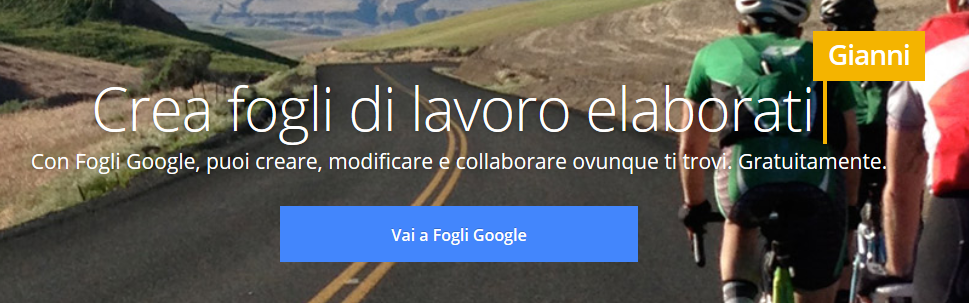
\includegraphics[height=0.3\textheight]{immagini/sheets.png}
\end{figure}
\footnotesize
\begin{itemize}
\item "Statistiche immediate"
\item "Funziona con Excel: non devi più preoccuparti dei formati dei file"
\end{itemize}
\end{frame}
\begin{frame}{Google Slides}
\begin{figure}[h!]

\includegraphics[height=0.3\textheight]{immagini/slides.png}
\end{figure}
\footnotesize
\begin{itemize}
\item "Presentazioni Google fa risaltare le tue idee con una varietà di temi per le presentazioni, centinaia di font, video incorporati, animazioni e altro ancora"
\item "Presenta facilmente le tue idee, senza bisogno di cavi. Presentazioni Google supporta Chromecast, Hangouts e AirPlay"
\item "Funziona con PowerPoint: non devi più preoccuparti dei formati dei file"
\end{itemize}
\end{frame}
\begin{frame}{Google Forms}
\begin{figure}[h!]

\includegraphics[height=0.3\textheight]{immagini/forms.png}
\end{figure}
\begin{figure}[h!]
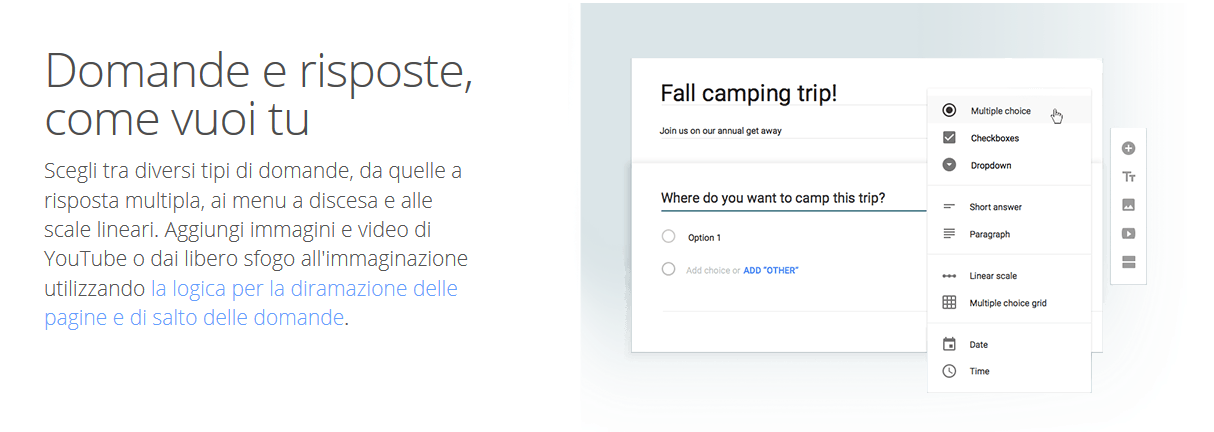
\includegraphics[width=\linewidth]{immagini/domande.png}
\end{figure}
\end{frame}

\subsection{Google Alerts}
\begin{frame}{Google Alerts}
\begin{figure}[h!]

\includegraphics[width = \linewidth]{immagini/alerts.jpg}
\end{figure}
\center Google Alerts è un servizio offerto da Google che notifica l'utente, tramite email, quando compaiono sul web articoli contenenti le parole chiave da lui indicate.
\end{frame}
\begin{frame}{Google Alerts}
\begin{columns}
\begin{column}{0.5\linewidth}
\begin{figure}[h!]
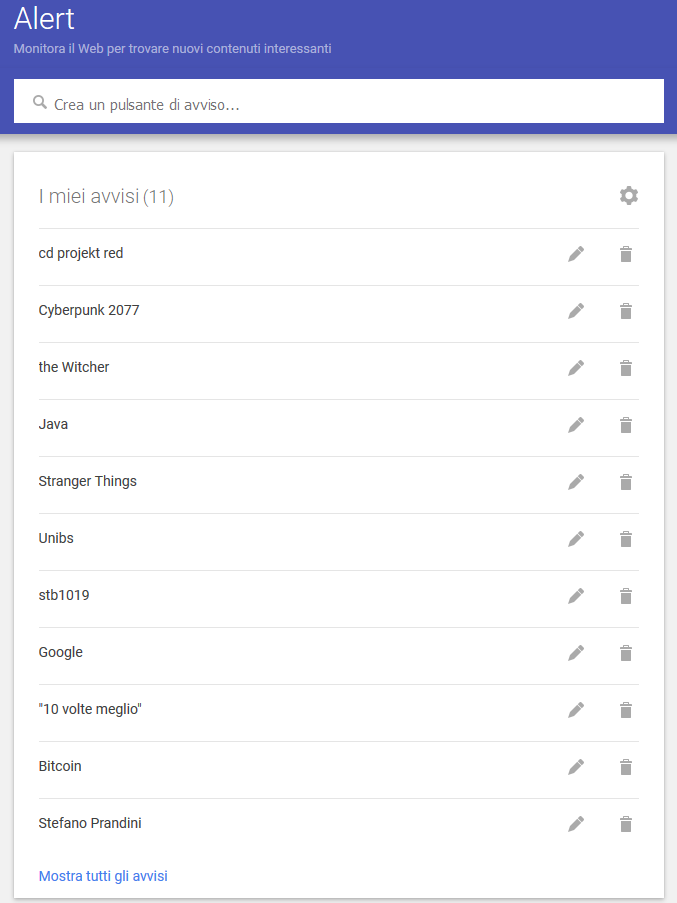
\includegraphics[height=0.8\textheight]{immagini/alert.png}
\end{figure}
\end{column}
\begin{column}{0.5\linewidth}
"Invece di fare tutto manualmente, dedicando molto del nostro tempo alla ricerca, basterà impostare degli “alerts” ed il tutto sarà più scorrevole, tanto da sembrare quasi di avere un assistente che ci invia delle e-mail ogni qual volta c’è una novità riguardo i termini (query) di ricerca che ci interessano."
\end{column}
\end{columns}
\end{frame}

\subsection{E tanto altro}
\begin{frame}{Calcolatrice}
\begin{figure}[h!]
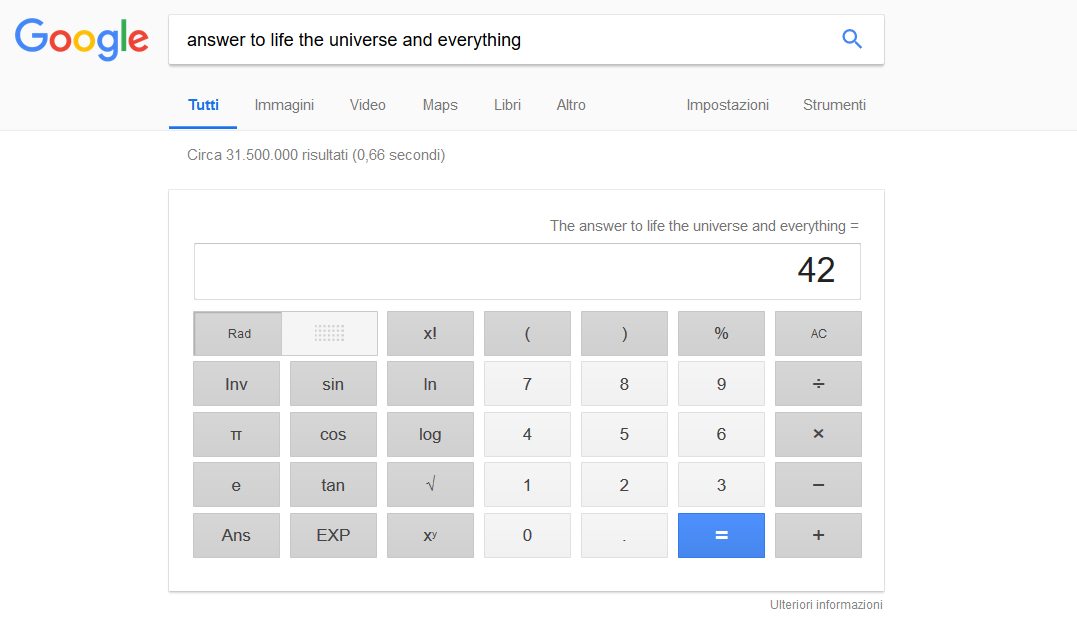
\includegraphics[width=\linewidth]{immagini/calc.png}
\end{figure}
\end{frame}
\begin{frame}{Funzioni}
\begin{columns}
\begin{column}{0.5\linewidth}
\begin{figure}[h!]
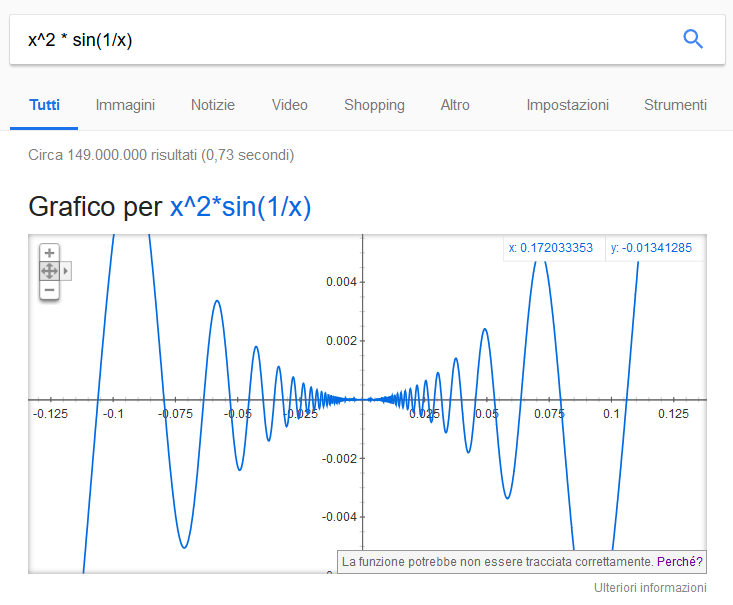
\includegraphics[width=\linewidth]{immagini/2d.png}
\caption{2D function}
\end{figure}
\end{column}
\begin{column}{0.5\linewidth}
\begin{figure}[h!]
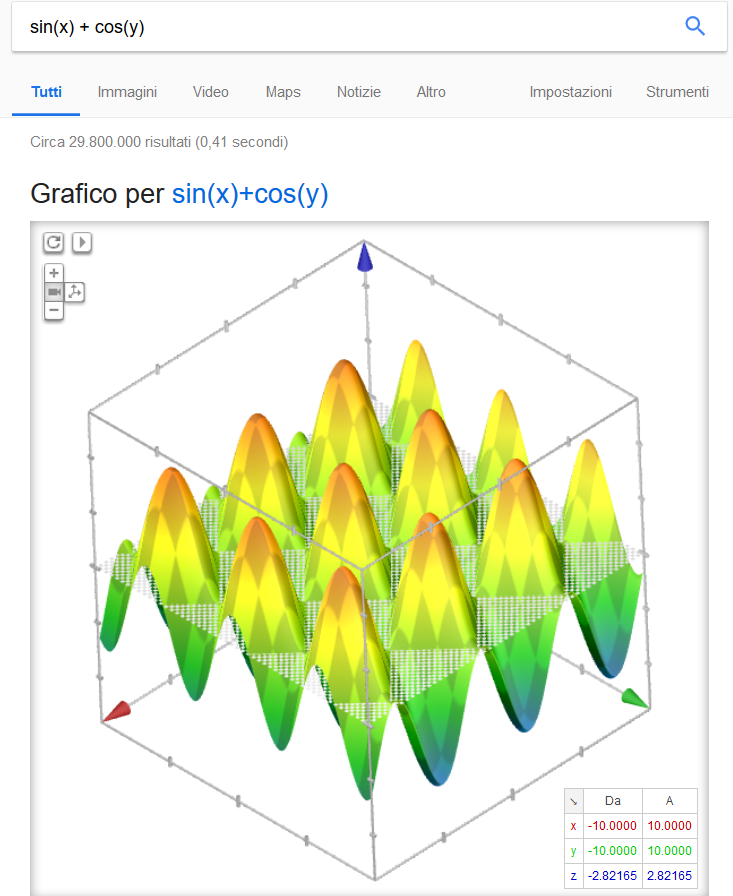
\includegraphics[height=0.7\textheight]{immagini/3d.png}
\caption{3D function}
\end{figure}
\end{column}
\end{columns}
\end{frame}
\begin{frame}{Selettore Colori}
\begin{columns}
\begin{column}{0.5\linewidth}
\begin{figure}[h!]
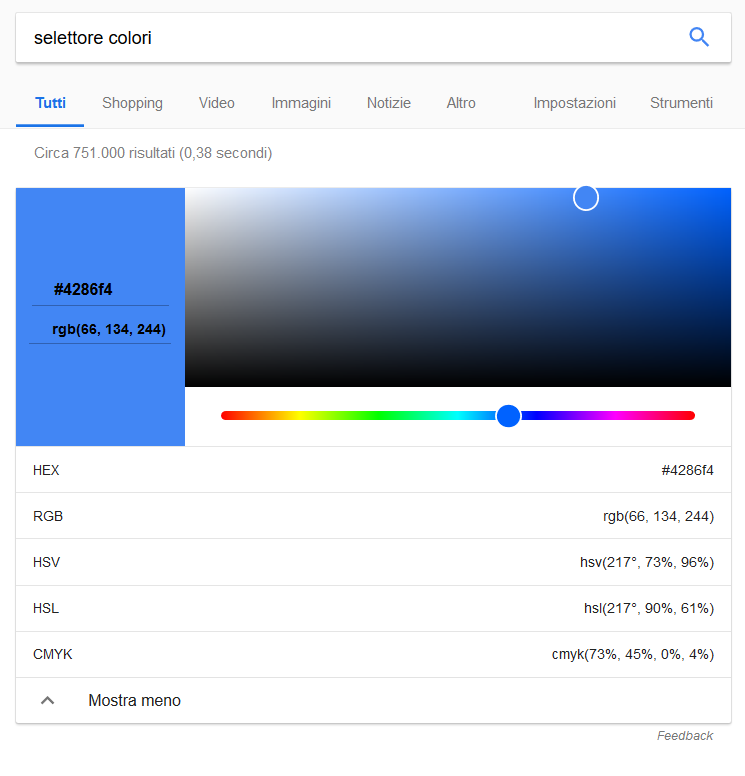
\includegraphics[width=\linewidth]{immagini/selettore.png}
\end{figure}
\end{column}
\begin{column}{0.5\linewidth}
\begin{figure}[h!]
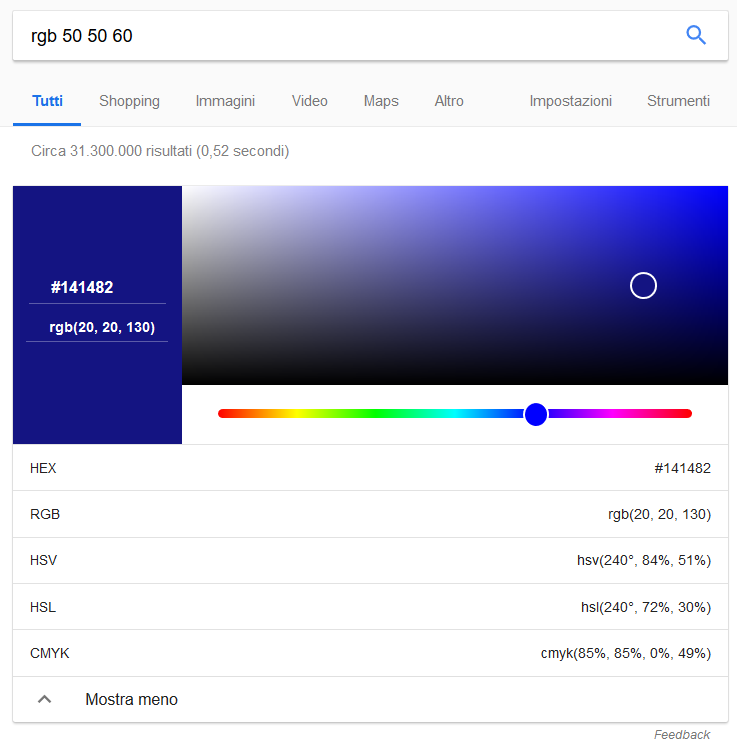
\includegraphics[width=\linewidth]{immagini/rgb.png}
\end{figure}
\end{column}
\end{columns}
\end{frame}

\begin{frame}{Ultimo ma non per importanza}
\begin{figure}[h!]

\includegraphics[height=0.6\textheight]{immagini/drive.png}
\caption{Questa presentazione è/sarà presente sul drive del Branch: sapete tutti come funziona?}
\end{figure}
\end{frame}

\begin{frame}{Domande? (uno alla volta per favore)}
\begin{figure}[h!]

\includegraphics[height=0.6\textheight]{immagini/help.jpg}
\end{figure}
\end{frame}

\begin{frame}{...E buon proseguimento di serata}
\begin{figure}[h!]

\includegraphics[height=0.6\textheight]{immagini/grazie.png}
\end{figure}
\center Stefano Prandini\\ \color{blue}{\underline{\href{mailto:stefano.prandini@ieee.org}{stefano.prandini@ieee.org}}}
\end{frame}





\end{document}